%%%%%%%%%%%%%%%%%%%%%%%%%%%%%%%%%%%%%%%%%%%%%%%%%%%%%%%%%%%%%%%%%%%%%%%%%%%%%%%%%%%%%%%%%%%%%%%%%%%%%%%%%%%%%%%%%%%%%%%%%%%%%%%%%%%%%%%%%%%%%%%%%%%%%%%%%%%
% This is just an example/guide for you to refer to when submitting manuscripts to Frontiers, it is not mandatory to use Frontiers .cls files nor frontiers.tex  %
% This will only generate the Manuscript, the final article will be typeset by Frontiers after acceptance.   
%                                              %
%                                                                                                                                                         %
% When submitting your files, remember to upload this *tex file, the pdf generated with it, the *bib file (if bibliography is not within the *tex) and all the figures.
%%%%%%%%%%%%%%%%%%%%%%%%%%%%%%%%%%%%%%%%%%%%%%%%%%%%%%%%%%%%%%%%%%%%%%%%%%%%%%%%%%%%%%%%%%%%%%%%%%%%%%%%%%%%%%%%%%%%%%%%%%%%%%%%%%%%%%%%%%%%%%%%%%%%%%%%%%%

%%% Version 3.4 Generated 2018/06/15 %%%
%%% You will need to have the following packages installed: datetime, fmtcount, etoolbox, fcprefix, which are normally inlcuded in WinEdt. %%%
%%% In http://www.ctan.org/ you can find the packages and how to install them, if necessary. %%%
%%%  NB logo1.jpg is required in the path in order to correctly compile front page header %%%

\documentclass[utf8]{frontiersSCNS} % for Science, Engineering and Humanities and Social Sciences articles
%\documentclass[utf8]{frontiersHLTH} % for Health articles
%\documentclass[utf8]{frontiersFPHY} % for Physics and Applied Mathematics and Statistics articles

%\setcitestyle{square} % for Physics and Applied Mathematics and Statistics articles
\usepackage{url,hyperref,lineno,microtype,subcaption,booktabs,amssymb,amsmath,multirow}
\usepackage[onehalfspacing]{setspace}

\linenumbers


% Leave a blank line between paragraphs instead of using \\


\def\keyFont{\fontsize{8}{11}\helveticabold }
\def\firstAuthorLast{Amaya {et~al.}} %use et al only if is more than 1 author
\def\Authors{Jorge Amaya\,$^{1,*}$, Romain Dupuis\,$^{1}$, Maria-Elena Innocenti$^{2}$ and Giovanni Lapenta\,$^{1}$}
% Affiliations should be keyed to the author's name with superscript numbers and be listed as follows: Laboratory, Institute, Department, Organization, City, State abbreviation (USA, Canada, Australia), and Country (without detailed address information such as city zip codes or street names).
% If one of the authors has a change of address, list the new address below the correspondence details using a superscript symbol and use the same symbol to indicate the author in the author list.
\def\Address{$^{1}$Centre for mathematical Plasma-Astrophysics, CmPA, Mathematics Department, KU Leuven, University of Leuven, Belgium \\
$^{2}$Jet Propulsion Laboratory, Interstellar and Heliospheric Physics Division, 4800 Oak Grove Dr, Pasadena, CA 91109, USA}
% The Corresponding Author should be marked with an asterisk
% Provide the exact contact address (this time including street name and city zip code) and email of the corresponding author
\def\corrAuthor{Jorge Amaya, Mathematics Department, Celestijnenlaan 200B, KU Leuven, 3001 Leuven, Belgium}

\def\corrEmail{jorge.amaya@kuleuven.be, jorgeluis.amaya@gmail.com}
\graphicspath{{figures/}}


\begin{document}

\onecolumn
\firstpage{1}

\title[Unsipervised classification of the solar wind]{Interpretable classification of the solar wind using unsupervised machine learning} 

\author[\firstAuthorLast ]{\Authors} %This field will be automatically populated
\address{} %This field will be automatically populated
\correspondance{} %This field will be automatically populated

\extraAuth{}% If there are more than 1 corresponding author, comment this line and uncomment the next one.
%\extraAuth{corresponding Author2 \\ Laboratory X2, Institute X2, Department X2, Organization X2, Street X2, City X2 , State XX2 (only USA, Canada and Australia), Zip Code2, X2 Country X2, email2@uni2.edu}


\maketitle


\begin{abstract}

%%% Leave the Abstract empty if your article does not require one, please see the Summary Table for full details.
\section{}
This is my abstract \citep{Roberts2020}.

This is the \href{https://github.com/murci3lag0}{link to my personal GitHub page}.

\tiny
 \keyFont{ \section{Keywords:} solar wind, ACE, Self-Organizing Maps, clustering, autoencoder, PCA, unsupervised, machine learning} %All article types: you may provide up to 8 keywords; at least 5 are mandatory.
\end{abstract}

\section{Introduction}
%The effects of solar activity on the magnetic environment of the Earth have been observed since the publication of Edward Sabine's work in 1852 \citep{Sabine1852}. During almost two hundred years we have learn about the intimate connection between our star and the plasma environment of the Earth. Three main physical processes connect the Sun to Earth: the transfer of electromagnetic radiation, the transport of energetic particles, and the flow of solar wind. The later is a continuous stream of charged particles that carries the solar magnetic field out of the corona and into the interplanetary space.

The name `solar wind' was coined by Parker in 1958 because `the gross dynamical properties of the outward streaming gas [from the Sun] are hydrodynamic in character'\citep{Parker1958}. Over time we have learned that the wind also has many more complex properties. Initially, it was natural to classify the solar wind by defining a boundary between `fast' and `slow' winds \citep{Habbal1997}. The former has been associated with mean speed values around 750 km/s, while the later shows a convincing limit at 500 km/s, where the compositional ratio (Fe/O) shows a significant break \citep{Feldman2005,Stakhiv2015}. The solar wind also carries information about its origins on the Sun. At certain solar distances the ion composition of the solar wind is expected to be frozen-in, reflecting the electron temperature in the corona and its region of origin \citep{Feldman2005,Zhao2009,Stakhiv2015}. These particles have multiple energies and show a variety of kinetic properties, including non-Maxwellian velocity distributions \citep{Pierrard2010,Matteini2012}.

The solar wind is also connected to the Sun by the Interplanetary Magnetic Field (IMF), thorough magnetic field lines directed towards the Sun, away from the Sun, or in the case of flux ropes connected at both ends \citep{Owens2016,Gosling2010}. The thin region where solar magnetic fields of opposite directions meet is called the Heliospherc Current Sheet (HCS). When a spacecraft crosses the HCS instruments onboard can detect the change in magnetic field direction as a 180$^\circ$ reversal. Changes in the flow properties are also observed around the HCS. This perturbed zone is called the Heliospheric Plasma Sheet (HPS), and the passage of the spacecraft from one side of the HPS to the other is known as a Sector Boundary Crossing (SBC) \citep{Winterhalter1994}. These are sometimes confused with Corotating Interaction Regions (CIR), which are zones of the solar wind where fast flows have caught up with slow downstream solar wind, compressing the plasma.

From the point of view of a spacecraft SBCs and CIRs can show similar sudden changes in the plasma properties of the solar wind. These two in turn are often grouped and mixed with other transient events, like Coronal Mass Ejections (CME) and Magnetic Clouds (MC). Since 1981 when \citep{Burlaga1981} described the propagation of MC behind an interplanetary shock, it was suspected that CMEs and MC where coupled. However, more recent studies show that CMEs observed near the Sun do not necessarily become MC, but instead `pressure pulses' \citep{Gopalswamy1998,Wu2006}.

Much more recently it has been revealed, by observations from Parker Solar Probe, that the properties of the solar wind can be drastically different closer to the Sun, where the plasma flow is more pristine and has not yet mixed with the interplanetary environment. Patches of large intermittent magnetic field reversals, associated with jets of plasma and enhanced Poynting flux, have been observed and named `switchbacks' \citep{Bale2019,Bandyopadhyay2020}.

The solar wind is thus not only an hydrodynamic flow, but a compressible mix of different populations of charged particles and electromagnetic fields that carry information of their solar origin (helmet streamer, coronal holes, filaments, solar active regions, etc.) and is the dominion of complex plasma interactions (ICMEs, MC, CIRs, SBCs, switchbacks).

To identify and study each one of these phenomena we have relied in the past on a manual search, identification and classification of spacecraft data. Multiple authors have created empirical methods of wind type identification based on in-situ satellite observations and remote imaging of the solar corona. Over the years the number and types of solar wind classes has changed, following our understanding of the complexity of heliospheric physics.

Solar wind classification serves three main roles:
\begin{enumerate}
	\item it is used for the characterization of its origins in the corona,
	\item to identify the conditions where the solar wind is geoeffective,
	\item to isolate different plasma populations in order to perform statistical analysis.
\end{enumerate}

Among these classifications we can include the original review work by \citep{Withbroe1986}, the impressive continuous inventory by \citep{Richardson2000,Richardson2010,Richardson2012}, and the detailed studies by \citep{Zhao2009} and \citep{Xu2015b}. These publications classify the solar wind based on its origins and on the transient events detected. Each system includes two, three or four classes, generally involving coronal-hole origins, CMEs, streamer belt origins and sector reversal regions.

We are moving now towards a new era of data analysis, where manual human intervention can be replaced by `intelligent' software. The trend has already started, with the work by \citep{Camporeale2017b} who used the \citep{Xu2015b} classes to train a Gaussian Process algorithm that autonomously assigns the solar wind to the proper class, and more recently by \citep{Roberts2020} who used unsupervised classification to perform a 4 and 8 class solar wind classification. Machine learning algorithms have been used in the past in other applications in solar physics \citep{Lundstedt1996,Qahwaji2008c,Ahmed2013c,Bobra2015,Bobra2016,Nishizuka2017c,Camporeale2018}, and astrophysics \citep{VanderPlas2012,Ntampaka2015,Hajian2015,Suveges2017,Bai2018,Bonjean2019}.

The most basic machine learning techniques learn using two methods: a) in supervised learning the algorithms are shown a group of inputs and ouputs with the goal to find a non-linear relationship between them, b) in unsupervised learning the machine is presented with a cloud of multi-dimensional points that have to be autonomously categorized in different classes. This means that we can program the computer to learn about the different types of solar wind using the existing empirical classifications, or by allowing it to independently detect patterns in the solar wind properties.

In the present work we show how the second method, unsupervised classification, can be used to segregate different types of solar wind. In addition, we show hot to visualize and interpret such results. The goal of this paper is to introduce the method to the community, the best use practices and the opportunities that such system can bring. We implement one specific type of classification, called Self-Organizing Maps, and we compare it to simpler classification techniques, showing that it can reveal hidden information in years of solar wind data.

In the next sections we present in detail the techniques of data processing (section \ref{}), data dimension reduction (section \ref{}) and data clustering (section \ref{}). We then present in detail the Self-Organizing Map technique and all its properties in section \ref{}. We show how to connect all of these parts together in section \ref{}, and finally we show how the full system can be used to study 15 years of solar wind data from the ACE spacecraft in section \ref{}.


%\citep{Gosling2010} : flux ropes, subset of CME, lasting ~12hours, low beta, smoothyl rotating.
%\citep{Wu2006} : MC duration of at least 8h
 
%/!\ for the tieme series figure: the HCS is generally easily identified by an approximately 180° change in direction of the magnetic field spiral angle over one to a few hours [Zhou et al., 2005]
%
%
%Magnetic reconnection solar wind-magnetosphere 1985
%
%
%Prediction model of solar wind geo-effectiveness using bayersian theory base on solar wind features 1997
%
%Geo-effectiveness of MCs, IPSs, and CIRs. 2011. CIRs alone in 2006
%
%Solar sources of geoeffective structures. Webb 2001. 
%
%Origins of the solar wind in the corona. Withbroe. Two clear sources: CH and CME. Role of streamers? role of things between? Role of spicules and polar plumes?
%
%Habbal, 1997: slow solar wind is associated with the axes, also known as stalks, of streamers. Furthermore, the ultraviolet observations also show how the fast solar wind is ubiquitous in the inner corona and that a velocity shear between the fast and slow solar wind develops along the streamer stalks
%
%Origin on the Sun of magnetic clouds and their structure: CME are flux ropes originating in filaments in the sun. 1986.
%
%** Solar wind properties and their effect on Earth. REVIEW of controversial and uncontroversial Solar sources: fast sw is from CH. Fast streams are known to be connected to the central regions of large coronal holes. Slow streams, however, appear to come from a wide range of sources, including streamers, pseudostreamers, coronal loops, active regions, and coronal hole boundaries. Forecasting techniques review. Cranmer 2017.
%--> Also: controversy about how to properly classify the sw.
%--> Also: solar wind features fade in time/distance --> Prepare for PSP!
%
%More detailed-recent classification using ACE: Coronal Sources and In Situ Properties of the Solar Winds Sampled by ACE During 1999 – 2008. Hui Fu 2015.

\section{Materials and Methods}

\subsection{Data and Processing}
\subsubsection{Data Set Used}
The solar wind data used in this work was obtained by the Advanced Composition Explorer (ACE) spacecraft, during a period of 14 years, between 1998 and 2011. The data can be downloaded from the \href{ftp://mussel.srl.caltech.edu/pub/ace/level2/multi}{FTP servers of The ACE Science Center (ASC)}. The files in this repository correspond to a compilation of hourly average data from three instruments: MAG (Magnetometer), SWEPAM (Solar Wind Electron, Proton, and Alpha Monitor) and EPAM (Electron, Proton, and Alpha Monitor). A detailed description of the entries in this data set can be found in the \href{http://www.srl.caltech.edu/cgi-bin/dib/rundibviewmultil2/ACE/ASC/DATA/level2/multi}{ASC website} listed in section \ref{sec:repos}.

A total of 122712 data points are available. However, routine maintenance operations, low statistics, instrument saturation and instrument degradation produce gaps and errors in the data. The SWICS data includes a flag assessing the quality of the calculated plasma moments. We retain only `Good quality' entries. Fig.\ref{fig:datacoverage} shows the final number of observations retained per year. Our pre-processed data set contains a total of 72454 points.

\subsubsection{Additional Derived Features}
We created additional features for each entry, based on previous knowledge of the physical properties of the solar wind. Some are derived from the existing properties in the data set, others computed from statistical analysis of their evolution.

Multiple techniques have been proposed in the literature to identify ejecta, Interplanetary Coronal Mass Ejections (ICME), and solar wind origins in the ACE data. \citep{Zhao2009} suggest that, during solar cycle 23, three classes of solar wind can be identified using its speed, $V_{sw}$, and the oxygen ion charge state ratio, $O^{7+}/O^{6+}$. The classification boundaries based on these three parameters are presented in Table \ref{tab:swtypes}. This solar wind classification will be known in this manuscript as the Z classification.
\citep{Xu2015b} suggested an alternative four class classification based on the proton-specific entropy, $S_p = T_p/n_p^{2/3}$, the Alfv\'en speed, $V_A = B / (\mu_0 m_p n_p)^{1/2}$, and the velocity-dependent expected proton temperature, $T_\text{exp} = (V_{sw}/258)^{3.113}$. The classification conditions based on these three parameters are also presented in Table \ref{tab:swtypes}. This solar wind classification will be known in this manuscript as the X classification\citep{Xu2015b}. For each entry in the data set we have included the values of $S_p$, $V_A$, $T_\text{exp}$, and the solar wind type given by the two classification methods. Additional auxiliary variables, like the Alfv\'en Mach number ($M_A$) and the temperature ratio ($T_\text{exp}/T_p$), have also been included in the data set.

In addition to these instantaneous quantities, we can perform statistical operations over a window of time of six hours, including values of the maximum, minimum, mean, standard deviation, variance, auto-correlation, and range. These quantities can be used to take into account temporal variations of the solar wind over the previous hours.

Two additional terms, which have been successfully used in the study of solar wind turbulence and wave characterization \citep{Zhao2018,Adhikari2020,Magyar2019}, are included here to account for additional time correlations: the normalized cross-helicity, $\sigma_c$ eq. \eqref{eq:sigmac}, and the normalized residual energy, $\sigma_r$ eq. \eqref{eq:sigmar}, where $\boldsymbol{b} = \left(\boldsymbol{B}- \boldsymbol{\left<B\right>}\right)/(\mu_0m_pn_p)^{1/2}$ is the fluctuating magnetic field in Alfv\'en units, $\boldsymbol{v} = \boldsymbol{V_{sw}}- \boldsymbol{\left<V_{sw}\right>}$ is the fluctuating solar wind velocity, $\boldsymbol{z^\pm} = \boldsymbol{v} \pm \boldsymbol{b}$ are the Els\"asser variables \citep{PhysRev.79.183}, and $\left<.\right>$ denotes the averaging of quantities over the time window.

\begin{align}
\sigma_c & = 2 \left< \boldsymbol{b}\cdot\boldsymbol{v}\right>/\left<\boldsymbol{b}^2 + \boldsymbol{v}^2\right> \label{eq:sigmac} \\
\sigma_r & = 2 \left< \boldsymbol{z^+}\cdot\boldsymbol{z^-}\right>/\left<\boldsymbol{z^-}^2 + \boldsymbol{z^+}^2\right> \label{eq:sigmar}
\end{align}

Due to gaps in the data, some of the above quantities can not be calculated. We eliminate from the data set all entries for which the derived features presented in this section could not be calculated. This leaves a total of 51608 entries in the data set used in the present work.

To account for the differences in units and scale, each feature column $\boldsymbol{F}$ in the data set is normalized to values between 0 and 1, using: $\boldsymbol{f}=\left(\boldsymbol{F}-\min{\boldsymbol{F}}\right) /\left(\max{\boldsymbol{F}}-\min{\boldsymbol{F}}\right)$.

\subsubsection{Complementary Data Catalogs}
We support the interpretation of our results using data from three solar wind event catalogs. The first is the well known Cane and Richardson catalog that contains information about ICMEs detected in the solar wind, ahead of the Earth \citep{Cane2003} \citep{Richardson2010} \footnote{\href{http://www.srl.caltech.edu/ACE/ASC/DATA/level3/icmetable2.htm}{Near-Earth Interplanetary Coronal Mass Ejections Since January 1996: http://www.srl.caltech.edu/ACE/ASC/DATA/level3/icmetable2.htm}}. We used the August 16, 2019 revision. As the authors state in their website, there is no spreadsheet or text version of this catalog and offline editing was necessary. We downloaded and re-formatted the catalog to use it in our application. The CSV file created has been made available in our repository. We call this, the Richardson and Cane catalog. 

The second catalog correspond to the ACE List of Disturbances and Transients\footnote{\href{http://www.ssg.sr.unh.edu/mag/ace/ACElists/obs\_list.html}{ACE Lists of Disturbances and Transients: http://www.ssg.sr.unh.edu/mag/ace/ACElists/obs\_list.html}} produced by the University of New Hampshire. As in the previous case, the catalog is only available as an html webpage, so we have manually edited the file and extracted the catalog data into a CSV file also available in our repository. This is here referred as the UNH catalog.


Finally, we also included data from the Shock Database\footnote{\href{https://www.cfa.harvard.edu/shocks/ac_master_data/}{Harvard-Smithsonian, Center for Astrophysics, Interplanetary Shock Database - ACE: https://www.cfa.harvard.edu/shocks/ac\_master\_data/}} maintained by Dr. Michael L. Stevens and Professor Justin C. Kasper at the Harvard-Smithsonian Center for Astrophysics. Once again we have gathered and edited multiple web-pages in a single CSV file available in our repository. In this work this last database will be known as the CfA catalog.

\subsection{Unsupervised classification}
\subsubsection{Dimension Reduction using PCA}
\label{sec:reducpca}
Principal Component Analysis (PCA) is a mathematical tool used in data analysis to simplify and extract the most relevant features in a complex data set. This technique is used to create entries composed of linearly independent `principal components'. These are the eigenvectors of the covariance matrix $\Sigma$ applied to the centered data, eq.\eqref{eq:covariance}, ordered from the largest to the smallest eigenvalue, $\lambda_1 \ge \lambda_2 \ge ... \ge \lambda_n$, where $\overline{\boldsymbol{X}}$ is the mean value of each original feature, eq.\eqref{eq:xmean}. The projection of the data onto the principal component space ensures a maximal variance on the direction of the first component. Each subsequent principal component is orthogonal to the previous ones and points in the direction of maximal variance in the residual sub-space \citep{Shlens2014}.

\begin{align}
\overline{\boldsymbol{X}} & = \frac{1}{m} \sum_{i=1}^{m} \boldsymbol{X}_i \label{eq:xmean} \\
\Sigma & = \frac{1}{m} \sum_{i=1}^{m} \left( \boldsymbol{X}_i - \overline{\boldsymbol{X}} \right)\left( \boldsymbol{X}_i - \overline{\boldsymbol{X}} \right) \label{eq:covariance}
\end{align}

The PCA transformation creates as many components in the transformed space, $\boldsymbol{\tilde{X}}$, as features in the original data space $\boldsymbol{X}$. However, components with small eigenvalues belong to a dimension where the variance is so small that it is impossible to separate points in the data. It is a general practice in data reduction to keep only the first $k$ components that explain at least a significant portion of the total variance of the data, $\lambda_{i=1..k}/\text{Tr}(\Sigma) > \epsilon$. This allows for a selection of information that will effectively differentiate data points, and for a reduction of the amount of data to process during analysis. Many techniques have been suggested for the selection of the values of $k$ and the cut-off $\epsilon$ \citep{Rea2016}. We use the value of $k=3$ to simplify the comparison among the different models, but for a detailed study of the solar wind, if a PCA transformation is applied, it is important to use a fixed criteria for the selection of the cut-offs.

Fig. \ref{fig:dimreduc} (A) is a 3D scatter plot of all the data points, colored by the Xu classification, projected on the first three PCA components. The features used to create this figure are presented in section \ref{sec:fourmodels}. Panel (B) contains the same data colored by the Zhao classification. These projections show that the Xu and Zhao classification are defined by hyper-planes separating the points, even if the data has been linearly transformed by the PCA. Class 2, ICMEs-ejecta, is restricted to a small domain in this coordinate system (for both the Xu and Zhao classification). The lateral plots on panel (A) are 2D histograms of the point distribution on the three main PCA planes. They show that the concentration of points is not homogeneous and different zones can be isolated using unsupervised classification techniques. There is a clear segregation of points in the (1st,2nd)-component plane: as we will see in subsequent sections, one of the features of the solar wind presents a strong bimodal distribution that is prioritized by the PCA.

\subsubsection{Dimension Reduction Using Autoencoders}
\label{sec:reducae}
PCA has a limitation: the principal components are a linear combination of the original properties of the solar wind. An alternative to data reduction is the use of autoencoders (AE). These are machine learning techniques that can create non-linear combinations of the original features projected on a latent space with less dimensions \citep{Hinton2006}. This is accomplished by creating a system where an encoding function, $\phi$, maps the original data $\boldsymbol{X}$ to a latent space, $\boldsymbol{\mathcal{F}}$, eq.\eqref{eq:encoder}. A decoder function, $\psi$, then maps the latent space back to the original input space, eq.\eqref{eq:decoder}. The objective of the autoencoder is to minimize the error between the original data and the data produced by the compression-decompression procedure as shown in eq.\eqref{eq:aeminimization}.

\begin{align}
\phi: & \boldsymbol{X} \rightarrow \boldsymbol{\mathcal{F}} \label{eq:encoder}\\
\psi: & \boldsymbol{\mathcal{F}} \rightarrow \boldsymbol{X} \label{eq:decoder} \\
\phi,\psi = & \underset{\phi,\psi}{\arg \min} \left\lVert \boldsymbol{X} - (\phi \circ \psi) \boldsymbol{X} \right\rVert^2 \label{eq:aeminimization}
\end{align}

Autoencoders can be represented as feed-forward neural networks, where fully connected layers lead to a central bottleneck layer with few nodes and then expands to reach again the input layer size. An encoded element, $\boldsymbol{z} \in \boldsymbol{\mathcal{F}}$, can be obtained from a data entry, $\boldsymbol{x} \in \boldsymbol{X}$, following the standard neural network function, eq.\eqref{eq:encodex}, where $\boldsymbol{W}$ is the weights matrix, $\boldsymbol{b}$ is the bias, and $\sigma$ is the non-linear activation function.

\begin{align}
\boldsymbol{z} & = \sigma \left( \boldsymbol{W}\boldsymbol{x} + \boldsymbol{b} \right) \label{eq:encodex} \\
\boldsymbol{\hat{x}} & = \sigma' \left( \boldsymbol{W'}\boldsymbol{z} + \boldsymbol{b'} \right) \label{eq:decodez} \\ 
\mathcal{L}(\boldsymbol{x}, \boldsymbol{\hat{x}}) & =  \left\lVert \boldsymbol{x}- \boldsymbol{\hat{x}} \right\rVert^2 \label{eq:aeloss}
\end{align}

The decoding procedure, shown in eq.\eqref{eq:decodez}, transforms $\boldsymbol{z}\rightarrow\boldsymbol{\hat{x}}$, where the prime quantities are associated with the decoder. The loss function, $\mathcal{L}(\boldsymbol{x}, \boldsymbol{\hat{x}})$, is the objective to be minimized by the training of the neural network using gradient descent. Once training is completed, the vector $\boldsymbol{z}$ is a projection of the input vector $\boldsymbol{x}$ onto the lower dimensional space $\boldsymbol{\mathcal{F}}$.

Additional enhancements and variations of this simple autoencoder setup exist in the literature, including multiple regularization techniques to minimize overfitting \citep{7407967}, Variational Autoencoders (VAE) that produce encoded Gaussian distribution functions \citep{Kingma2013}, and Generative Adversarial Networks (GAN) that produce new (unseen) data \citep{Goodfellow2014}. In this work we use the most basic form of autoencoders, presented above.

The second column of Fig.\ref{fig:dimreduc}, panels (C) and (
D), contains the same information as the first column, but with the data set encoded in the three dimensional latent space $\boldsymbol{\mathcal{F}}$. Panel (C) shows that all the classes in the Xu and Zhao classification are easy to distinguish, including ICMEs-ejecta (class 2) that is difficult to discern in the PCA. This projection also shows that class 4 from the Zhao classification in the bottom panels, overlaps with class 3 (sector reversal origin), and partially with class 2 (ejecta) in the Xu classification on the top panels. Panel (C) shows, on the side planes, 2D histograms of the density of points. These can be seen as the volume integral of the point density in each direction. Here again it is possible to observe multiple zones of high concentration, suggesting that multiple types of solar wind are present in the data and that they can be differentiated using an unsupervised classification technique. 

\subsubsection{Clustering Techniques}
\label{sec:clustering}
The goal of unsupervised machine learning is to group data points in a limited number of clusters in the N-dimensional space $\Omega\in\Bbb R^N$, where N is the number of features (components or properties) in the data set. Multiple techniques can be used to perform multi-dimensional clustering. We present in Fig. \ref{fig:clustering} the three clustering techniques used to classify our 3D reduced data. The panels in the first column show the data projected in the PCA reduced space, $\boldsymbol{\tilde{X}}$, while the second column shows the data in the latent AE space, $\boldsymbol{\mathcal{F}}$. Each row corresponds to a different clustering method. The colors in the top panels (A) and (D) were obtained using the $k$-means method \citep{1056489}, the colors in the middle panels (B) and (E) were obtained using the Gaussian Mixture Model (GMM) \citep{bishop2006machine}. The bottom panels are colored by the classes from the Self-Organizing Maps described later in section \ref{sec:som}.

The $k$-means technique has already been used in a recent publication for the determination of solar wind states \citep{Roberts2020}. To our knowledge other clustering methods have never been used in the literature to classify the solar wind, but \citep{Dupuis2020} has used the GMM to characterize magnetic reconnection regions in simulations using their velocity distribution information.

The colors used in Fig.\ref{fig:clustering} are assigned randomly by each clustering technique. The most glaring issue with them is that different methods can lead to different clusters of points. The GMM and the $k$-means agree on their classification in the PCA space, but show dissimilar results in the AE space. Moreover, for a single method, e.g. $k$-means, slight modifications of the clustering parameters, e.g. using a different seed for the random number generator, can lead to very different results. We address this last issue using an algorithm that launches the $k$-means and GMM algorithms 500 times until the methods converge to a quasi-steady set of clusters. But we warn that the results are implementation dependent.

In the present data set, the cloud of points is convex and well distributed in all three components. This raises one additional issue, observed more clearly in the first column of Fig.\ref{fig:clustering}: when classical clustering methods are applied to relatively homogeneously dense data, it divides the feature space in Vorono\"i regions with linear hyper-plane boundaries. This is an issue with all clustering techniques based on discrimination of groups using their relative distances (to a centroid or to the mean of the distribution). To avoid this problem density-based techniques, such as DBSCAN \citep{ester1996density}, and agglomeration clustering methods, use a different approach. However, we can not apply them here because in such homogeneous cloud of points these techniques lead to a trivial solution where all data points are assigned to a single class.

There is no guarantee that a single classification method, with a particular set of parameters will converge to a physically meaningful classification of the data if the points in the data do not have some level of separability, or have multiple zones of high density. This is also true for other classification methods based on `supervised learning'. In those applications same issues will be observed if the training data uses target classes derived from dense data clouds using simple hyper-plane boundaries, as done for the Zhao and Xu classes. An example of such application was published by \citep{Camporeale2017b}. The authors used the Xu classification to train a Gaussian Process classifier.

\subsubsection{Self-Organizing Maps}
\label{sec:som}

\paragraph{Classical SOM}

Following the definitions and notations by \citep{Villmann2006}, a class can be defined as $C_i\overset{\text{def}}{=} \{x\in\Omega | \Phi(x)=\boldsymbol{w}_i\}$, where $\Phi$ is a function from $\Omega$ to a finite subset of $k$ points $\{\boldsymbol{w}_i\in\Bbb R^N\}_{i=1..k}$. A cluster $C_i$ is then a partition of $\Omega$, and $\{\boldsymbol{w}_i\}$ are the code words (also known as nodes, weights or centroids) associated. The mapping from the data space to the code word set, $\Phi: \Omega\rightarrow\mathcal{W}$, is obtained by finding the closest neighbor between the points $\boldsymbol{x}$ and the code words $\boldsymbol{w}$, eq.\eqref{eq:winner}. The code word $\boldsymbol{w_s}$, the closest node to the input $\boldsymbol{x_s}$, is called the `winning element'. The class $C_i$ corresponds to a Vorono\"i region of $\Omega$ with center in $\boldsymbol{w}_i$.

\begin{equation}
\Phi: x \rightarrow  \underset{i\in\mathcal{N}}{\arg\min}\left( \left\lVert x - \boldsymbol{w}_i \right\rVert \right) \label{eq:winner}
\end{equation}

A Self-Organizing Map (SOM) also composed of structured nodes arranged in a lattice, and assigned to a fixed position $\boldsymbol{p}_i$ in $\Bbb R^q$, where $q$ is the dimension of the lattice (generally $q=2$). The map nodes are characterized by their associated code words. The SOM learns by adjusting the code words $\boldsymbol{w}_i$ as input data $x$ is presented.

The SOM is the ensemble of code words and nodes $A_i = \{ \boldsymbol{w}_i, \boldsymbol{p}_i\} \in (\Omega \times \Bbb R^q)$. For a particular entry $\boldsymbol{x_s}$, the code word $s \in \mathcal{N}$ is associated to the winning node $\boldsymbol{p_s}$ if the closest word to $\boldsymbol{x_s}$ is $\boldsymbol{w_s}$. At every iteration of the method, all code words of the SOM are shifted towards $x$ following the rule:

\begin{equation}
\Delta \boldsymbol{w}_i = \epsilon(t)h_\sigma(t,i,s)(x-\boldsymbol{w}_i) \label{eq:learnsom}
\end{equation}

with $h_\sigma(t,i,j)$ defined as the lattice neighbor function:

\begin{equation}
h_\sigma(t,i,j) = e^{-\frac{\left\lVert \boldsymbol{p}_i - \boldsymbol{p}_j \right\rVert^2}{2\sigma^2(t)}} \label{eq:neigsom}
\end{equation}

where $\epsilon(t)$ is the time dependent learning rate, eq.\eqref{eq:epsilon}, and $\sigma(t)$ is the time dependent lattice neighbor width, eq.\eqref{eq:sigma}. The training of the SOM is an iterative process where each data point in the data set is presented to the algorithm multiple times $t={0, 1,..,t_f}$. In these equations the subscript $0$ refers to initial values at $t=0$ and the subscript $f$ to values at $t=t_f$.

\begin{align}
\epsilon(t) & = \epsilon_0 \left(\frac{\epsilon_f}{\epsilon_0}\right)^{t/t_f} \label{eq:epsilon} \\
\sigma(t) & = \sigma_0 \left(\frac{\sigma_f}{\sigma_0}\right)^{t/t_f} \label{eq:sigma}
\end{align}

This procedure places the code words in the data space $\Omega$ in such a way that neighboring nodes in the lattice are also neighbors in the data space. The lattice can be presented as a $q$-dimensional image, called map, where nodes sharing similar properties are organized in close proximity.

The main metric for the evaluation of the performance of the SOM is called the quantization error:

\begin{equation}
Q_E = \frac{1}{M} \sum_{i=1}^M \left\lVert x_i - w_{x_i} \right\rVert
\end{equation}

where $M$, is the total number of entries in the data set.

Once the training of the SOM is finished, the code words $\boldsymbol{w}_i$ can be grouped together using any clustering technique, e.g. k-means. The nodes of the SOM with close properties will be made part of the same class. The classes thus created are an ensemble of Vorono\"i subspaces, allowing a complex non-linear partitioning of the data space $\Omega$.

The final number of clusters is an input of the algorithm, but can also be calculated autonomously. The Within Cluster Sum of Squares (WCSS) can be used as a metric of the compactness of the clustered nodes. As its name implies the WCSS is the sum of the squred distances from each node to their cluster point. If only one class is selected, the large spread of the nodes would produce a high WCSS. The lowest possible value of the WCSS is obtained for a very high number of classes, when the number of classes is equal to the number of nodes. But such extreme solution is also unpractical. The optimal number of clusters can be obtained using the Kneedle class number determination \citep{5961514}. In the present work we do not use this technique: we will perform comparisons with previous publications that propose a fixed number of solar wind types. We will explore the use of an automatic class number selection in a future publication.

\paragraph{Dynamic SOM}
The time dependence of the SOM training allows the code words $\boldsymbol{w}_i$ to reach steady coordinates by slowing down their movement over the iterations. Due to the minimization of the distance in eq.\eqref{eq:winner} code words tend to agglomerate around high density zones of the feature space. The Dynamic Self-Organizing Map (DSOM), introduced by \citep{Rougier2011}, eliminate the time dependence and allows to cover larger zones of the space outside of the high density regions.

The DSOM is a variation of the SOM where the learning function \eqref{eq:learnsom} and the neighbor function \eqref{eq:neigsom} are replaced by eqs. \eqref{eq:learndsom} and \eqref{eq:neigdsom} respectively:

\begin{align}
\Delta \boldsymbol{w}_i & = \epsilon \left\lVert x - \boldsymbol{w}_i \right\rVert_\Omega h_\eta(i,s,x)(x-\boldsymbol{w}_i) \label{eq:learndsom} \\
h_\eta(i,s,x) & = e^{-\frac{1}{\eta^2}\frac{\left\lVert \boldsymbol{p}_i - \boldsymbol{p}_j \right\rVert^2}{\left\lVert x - \boldsymbol{w}_s \right\rVert_\Omega^2}} \label{eq:neigdsom} 
\end{align}

where $\epsilon$ is a constant learning rate, $h_\eta(i,s,x)$ is defined as the new lattice neighbor function, and $\eta$ is the `elasticity' parameter. In their work \citep{Rougier2011} show that DSOM can be used to better sample the feature space $\Omega$, reducing the agglomeration of code words around high density zones. The DSOM does not converge to a steady solution, due to the lack of a temporal damping factor.

\paragraph{Visualization of SOM and DSOM}
Clustering techniques do not necessarily convergence to a steady immutable solution. Differences in the training parameters or slight changes in the data can have an important impact on the final classification. These tools can be used for statistical analysis, comparisons, data visualization and training of supervised methods. But it will be practically impossible to claim the existence of a general objective set of states discovered only by the use of these basic clustering techniques.

However, SOMs and DSOMs provide an important tool for the study of the solar wind: the maps are composed of nodes that share similar properties with its immediate neighbors. This allows for visual identification of patterns and targeted statistical analysis.

Fig.\ref{fig:maps} shows the basic types of plots and maps that can be generated using the SOM/DSOM techniques. This figure uses data from the model Amaya-21 which has been encoded, using AE, into a set of entries, $\boldsymbol{z}_i$, each one composed of three components. Panel (A) shows a histogram of the first two components of the feature space $\Omega$, with dots marking the position of the code words $\boldsymbol{w}_i$. The colors of the dots represent their SOM classification. The red lines connect a single code word $\boldsymbol{w}_s$ with its six closest neighbors. The panel (B) shows the `hit map' of the SOM. It contains the lattice nodes $\boldsymbol{p}_i$ associated to the code words $\boldsymbol{w}_i$. They are depicted as hexagons with sizes representing the number of data points connected to each node and colored by their SOM class. The thickness of the lines between lattice nodes represent the relative distance to its neighbors in the feature space $\Omega$. Red lines connect the node $\boldsymbol{p}_s$, associated to the code word $\boldsymbol{w}_s$ in panel (A), to its closest neighbors.

Panel (C) of Fig.\ref{fig:maps} corresponds to the value of a single feature associated to each node; as an example we use the ionized oxygen ratio $O^{7+}/O^{7+}$ (`O7to6'). To improve visualization all hexagon sizes have been set to their maximum and the inter-node distance line has been colored white. In order to obtain the correct value for each node, we must first perform a decoding of the data from the latent space, $\Omega=\boldsymbol{\mathcal{F}}$, to the original data set space, $\boldsymbol{X}$.

Panel (D) of Fig.\ref{fig:maps} shows that the nodes of the lattice can also be used to present data that has not been used in the training of the SOM. The method keeps track of the points in the data set associated to each lattice node, it is then possible to perform independent statistical operations on those points alone. Moreover, it is possible to activate the SOMs with just a subset of the data, i.e. with points that feature a specific solar wind type. In this case, as an example, we have colored the map using the average oxygen charge state $\left<Q_{O}\right>$ (`avqO'), and we have set the size of the nodes to represent the frequency of points with solar wind type Xu=2 (ejecta). The dark line between the lattice nodes designate the boundaries between different SOM classes.

These four representations are only a few examples of the variety of data that can be represented using SOMs. The most important aspect of the SOMs is that data is represented in simple 2D lattices where the nodes share properties with their neighbors. Here we also decided to use hexagonal nodes, connecting 6 equidistant nodes, but other types of representations are also valid, e.g. squared or triangular nodes.

The bottom row of Fig.\ref{fig:maps} displays all three components of the code words $\boldsymbol{w}_i$ associated with each one of the $\boldsymbol{p}_i$ nodes. In the first panel they have been mapped to the basic colors Red, Green and Blue (RGB). The remaining panels have been colored using each individual component. The first panel is then the RGB composition of the three remaining ones where the boundaries between the SOM classes have been highlighted.

\subsubsection{The Full Architecture}
\label{sec:fullarchi}
The previous sections introduced all the individual pieces that we use for the present work. Here we give a global view of the full model. Fig.\ref{fig:architecture} shows how all the components are interconnected. The data set is composed of clean and processed entries. We tested the PCA transformation in cases Amaya-21 and Roberts-8, keeping only the first three principal components. This possible setup is presented on the left of the figure. It is also possible to perform an unsupervised clustering directly on the un-processed data, as shown on the top of the figure, but it is not recommended. For the remaining of this manuscript we present only the cases where the non-linear AE encoding, shown at the right of Fig.\ref{fig:architecture}. The bottleneck of the AE network is three nodes, i.e. the data is encoded in three components. The transformed data is then used to train the SOM.

After training, the code words of the SOM are then clustered to group together nodes that share similar properties. This second level classification is done using the $k$-means++ algorithm with 500 re-initializations (it is in general recommended to use between 100 and 1000 iterations). The total number of classes selected is an input of the model and has been set to 8. This arbitrary choice was made following the results presented by \citep{Roberts2020}. All the software was implemented in Python using as main libraries PyTroch, Scikit-learn and Pandas.

\paragraph{Autoencoder architecture}
We use a basic, fully connected feed-forward neural network for the encoding-decoding process. The bottleneck of the network has been fixed to three neurons in order to simplify the visualization. This arbitrary choice is another parameter of the models that need further investigation. The neural network is symmetric in size but the weights of the encoder, $\boldsymbol{W}$, and the decoder, $\boldsymbol{W'}$, are not synchronized (see eqs.\eqref{eq:encodex}, \eqref{eq:decodez}). We use multiple fully connected hidden layers, where the central layer is the size of the bottleneck. Each layer is composed of a linear regressor, followed by batch normalization and a ReLU activation function. The output layer of the network contains a linear regressor followed by a hyperbolic tangent activation function. The autoencoder has been coded in python using the PyTorch framework.

We use an Adam optimizer \citep{Kingma2014} for the gradient descent with a learning rate of 0.001 and a weight decay of 0.0001 for regularization. The loss function is the Mean Squared Error (MSE). We train the network for 30 epochs, after which we see no additional improvement in the loss function. The full data set was randomly divided 50\%/50\% between training and testing sets.

\paragraph{Two Models of Solar Wind Classification}
\label{sec:fourmodels}
We have tested the two models presented in Table \ref{tab:features}. The models are inspired by the work of \citep{Roberts2020}. We call these cases Amaya-21 and Roberts-8.  The table lists all the features used in each model. A detailed description of each feature can be found in the \href{http://www.srl.caltech.edu/cgi-bin/dib/rundibviewmultil2/ACE/ASC/DATA/level2/multi}{ACE Level 2 documentation}. To spread the data over a larger range of values in each component, we have used the logarithm of all the quantities, except of those marked with an asterisk in the table.

Features 15 to 20 contain an additional suffix, corresponding to a statistical operation performed on the corresponding feature. The operations include the mean, the range, the standard deviation and the auto-correlation of quantities over a window of time of 6 hours. This window allows to capture temporal (spatial) fluctuations in some of the solar wind parameters.

On the lower part of Table \ref{tab:features} we present the range of dates used for each model. For Amaya-21 we use the full data set, while for the model Roberts-8 we try to replicate as much as possible the choices made in \citep{Roberts2020}. The same table also contains the hyper-parameters selected to run the two models. The number of neurons per layer in the encoding half of the neural network is listed in the table and was manually selected to minimize the final loss value of the AE.

All the figures presented until now correspond to the processing of data from model Amaya-21. The amount of data and figures produced in this work is very large and is not possible to include all of them in the present document. We will present in the next section some highlights, but more detailed analysis of each one of the cases will be presented in future publications.

\paragraph{Budget}
Machine learning models require fine tuning of different parameters, from the selection and testing of multiple methods, to the parameterization of the final architecture. \citep{Dodge2019} suggests that every publication in machine learning should include a section on the budget used for the development and training of the method. The budget is the amount of resources used in the data processing, the selection of the model hyper-parameters (HP), and its training.

The most time-consuming task in the present work has been the data preparation, the model setup and debugging and the writing of the SOM visualization routines. All the techniques described in the previous sections have been coded in python and are freely accessible in the repositories listed in section \ref{sec:repos}. We estimate the effort to bring this work from scratch to a total of 2 persons month. Of these, one person week was dedicated to the manual testing an selection of different model HPs (autoencoder architecture, feature selection, learning rates, initialization methods, number of epochs for training, selection of data compression method, size of the time windows, etc.).

All classic clustering techniques presented in section \ref{sec:clustering} require only a few lines of code and can be trained in minutes on a mid-range workstation (e.g. Dell Precission T5600, featuring two Intel(R) Xeon(R) CPU E5-2643 0 @ 3.30GHz with four cores and eight threads each). The most time consuming tasks of our models are the training of the autoencoder (5\% od the total run time), the multiple passages of the clustering algorithms (15\% of the run time), and the optimization of the SOM hyper-parameters (80\% of the run time). The training of the SOM is performed in less than a minute.

For reference, the total run-time for each one of the models used in this work are: 60 minutes for the Amaya-21 model and 20 minutes for the Roberts-8 model.

\paragraph{Hyper-Parameter Optimization}
Our main goal in this manuscript is to introduce the use of the SOMs for the classification of solar wind data. SOMs require the selection of four main Hyper-Parameters (HPs): the size of the lattice, $(m\times n)$, the initial learning rate, $\epsilon_0$, and the initial neighbor radius, $\sigma_0$. In the case of the DSOM algorithm, these two last HPs are replaced by the constant learning rate, $\epsilon$, and the elasticity, $\eta$. The automatic selection of the best HP for machine learning model is called Hyper-Parameter Optimization (HPO).

We use the library `optuna' \citep{Akiba2019} to perform an automatic optimization of the four HPs. The optimization is based on a technique called Tree-structured Parzen Estimator (TPE) \citep{pmlr-v28-bergstra13}. The objective function of the optimizer was set to minimize the expression:

\begin{equation}
\mathcal{H}\left(\sigma, \eta, m, n\right) = Q_E(\sigma, \eta, m, n) + \alpha \frac{m}{m_{max}} + \beta \frac{n}{n_{max}} + \gamma m n \label{eq:hpo}
\end{equation}

where $Q_E$ is the SOM quantization error, $m$ and $n$ are the number of lattice nodes in each dimension, and $m_{max}$ and $n_{max}$ are the given maximum number of possible nodes. The weight factors $\alpha$, $\beta$ and $\gamma$ are used to impose more or less restictions on each term. This optimization objective allows to minimize the quantization error, but also the number of nodes in the SOM. The squaring term $\gamma m n$ forces the map to be as squared as possible.

After a total of 100 trial runs of the model using different HPs, the optimizer selected the parameters presented in the lower section of table \ref{tab:features}. The total run time for the HPO of the case Amaya-21 is about 40 minutes. HPO is, understandably, one of the most expensive procedures in all our setup.

\subsection{Model Hyper-Parameter Selection}
\paragraph{Budget}
Machine learning models require fine tuning of different parameters, from the selection and testing of multiple methods, to the parameterization of the final architecture. \citep{[REF??]} suggests that every publication in machine learning should include a section on the budget used for the development and training of the method. The budget is the amount of resources used in the data processing, the selection of the model hyper-parameters (HP), and its training.

The most time-consuming task in the present work has been the data preparation, the model setup and debugging and the writing of the SOM visualization routines. All the techniques described in the Methods section \ref{sec:methods} have been coded in python and are freely accessible in the repositories listed in section \ref{sec:repos}. We estimate the effort to bring this work from scratch to a total of 2 persons month. Of these, one person week was dedicated to the testing an selection of different model HPs (autoencoder architecture, feature selection, learning rates, initialization methods, number of epochs for training, selection of data compression method, size of the time windows, etc.).

All classic clustering techniques presented in section \ref{sec:clustering} require only a few lines of code and can be trained in less than a minute on a current generation laptop (e.g. Dell XPS 13 2016 with an Intel Core i7-7500U CPU). The most time consuming task is the training of the autoencoder which can last for up to 3 minutes. The training of the SOM is performed in less than a minute.

\paragraph{Hyper-Parameter Optimization}
We are focusing in this work on the use of the SOMs. These require the selection of four main HPs: the size of the lattice, $(m\times n)$, the initial learning rate, $\epsilon_0$HPs are replaced by the constant learning rate, $\epsilon$, and the elasticity, $\eta$. The automatic selection of the best HP for machine learning model is called Hyper-Parameter Optimization (HPO).

We use the library `optuna' \citep{[REF??]} to perform an automatic optimization of the four HPs. The optimization is based on a technique called Tree-structured Parzen Estimator (TPE) \citep{[REF 3 IN OPTUNA PAPER??]}. The objective function of the optimizer was set to minimize the quantization error $Q_E$, the mean inter nodal distance, and the elasticity (or the neighborhood width) of the SOM. After a total of 100 trials (runs of the model using different HPs), the optimizer selected the parameters presented in table \ref{tab:hpo}. The total run-time for a single HPO is in the order of 30 minutes on a home computer. HPO is, understandably, the most expensive procedure.

\section{Results and comparisons}
Fig. \ref{} shows a schematic of the model used in the present work. Each entry in the ACE data set is encoded (or 


\section{Discussion}
This is the discussion.

\section{Additional Requirements}

\section*{Conflict of Interest Statement}
%All financial, commercial or other relationships that might be perceived by the academic community as representing a potential conflict of interest must be disclosed. If no such relationship exists, authors will be asked to confirm the following statement: 

The authors declare that the research was conducted in the absence of any commercial or financial relationships that could be construed as a potential conflict of interest.

\section*{Author Contributions}

The Author Contributions section is mandatory for all articles, including articles by sole authors. If an appropriate statement is not provided on submission, a standard one will be inserted during the production process. The Author Contributions statement must describe the contributions of individual authors referred to by their initials and, in doing so, all authors agree to be accountable for the content of the work. Please see  \href{http://home.frontiersin.org/about/author-guidelines#AuthorandContributors}{here} for full authorship criteria.

\section*{Funding}

JA has received funding from the European Union’s Horizon 2020 research and innovation programme under grant agreement No 754304 (\href{https://www.deep-projects.eu}{DEEP-EST, www.deep-projects.eu}).

RD has received funding from the European Union’s Horizon 2020 research and innovation programme under grant agreement No 776262 (\href{https://www.aida-space.eu}{AIDA, www.aida-space.eu}).

\section*{Acknowledgments}
The authors would like to acknowledge the help of D. Aaron Roberts (NASA, GSFC).

\section*{Supplemental Data}
Codes can be found in the \href{http://github.com/murci3lag0}{github.com/murci3lag0}.

\section*{Data Availability Statement}
\label{sec:repos}

Publicly available datasets were analyzed in this study. This data can be found here: \href{http://github.com/murci3lag0}{github.com/murci3lag0}.

The original contributions presented in the study are publicly available. This data can be found here: \href{http://github.com/murci3lag0}{github.com/murci3lag0}.

ACE datasets downloaded from \href{ftp://mussel.srl.caltech.edu/pub/ace/level2/multi}{ftp://mussel.srl.caltech.edu/pub/ace/level2/multi}.

ACE multi-instrument data set description: \href{http://www.srl.caltech.edu/cgi-bin/dib/rundibviewmultil2/ACE/ASC/DATA/level2/multi}{http://www.srl.caltech.edu/cgi-bin/dib/rundibviewmultil2/ACE/ASC/DATA/level2/multi}

Sunspots from \href{http://www.sidc.be/silso/datafiles}{http://www.sidc.be/silso/datafiles}

% Please see the availability of data guidelines for more information, at https://www.frontiersin.org/about/author-guidelines#AvailabilityofData

\bibliographystyle{frontiersinSCNS_ENG_HUMS} % for Science, Engineering and Humanities and Social Sciences articles, for Humanities and Social Sciences articles please include page numbers in the in-text citations
%\bibliographystyle{frontiersinHLTH&FPHY} % for Health, Physics and Mathematics articles
\bibliography{swinsom}

%%% Make sure to upload the bib file along with the tex file and PDF
%%% Please see the test.bib file for some examples of references

\section*{Tables}

\begin{table}\centering
	\begin{tabular}{@{}llll@{}}
		\toprule
		\# & Solar wind type name & Condition & Reference \\
		\midrule
		1 & Coronal hole wind & $O^{7+}/O^{6+} \leq 0.145$ & \citep{Zhao2009} \\
		2 & ICMEs & $O^{7+}/O^{6+}\leq 6.008e^{(-0.00578V_{sw})}$ & \\
		4 & Non-coronal hole wind & $0.145 < O^{7+}/O^{6+} < 6.008e^{(-0.00578V_{sw})} $ & \\
		\midrule
		0 & Streamer belt origin & Not type 1, 2, or 3 & \citep{Xu2015} \\
		1 & Coronal hole origin & Not type 2, and & \\
		  &  & $\log_{10}(S_p) > -0.525 \log_{10}(T_{\text{exp}}/T_p) - 0.676\log_{10}(V_A) + 1.74$ & \\
		2 & Ejecta & $\log_{10}(V_A) > 0.055\log_{10}(T_{\text{exp}}/T_p) + 0.277 \log_{10}(S_p) + 1.83$ & \\
		3 & Sector reversal origin & Not type 2, and & \\
		  & & $\log_{10}(S_p) < -0.125 \log_{10}(T_{\text{exp}}/T_p) - 0.658\log_{10}(V_A) + 1.04$ &  \\
		\bottomrule
	\end{tabular}
	\caption{The four solar wind types, as defined by \citep{Zhao2009} (top) and \citep{Xu2015} (bottom).}
	\label{tab:swtypes}
\end{table}

\begin{table}\centering
	\begin{tabular}{@{}lcccc@{}}
		\toprule
		Method & $m$ & $n$ & $\epsilon$ & $\sigma$ or $\eta$ \\
		\midrule
		\multirow{4}{*}{SOM} & v1 & v2 \\
						  	  & v3 & v4 \\
						  	  & v3 & v4 \\
						  	  & v3 & v4 \\
		\midrule
		\multirow{4}{*}{DSOM} & v1 & v2 \\
							   & v3 & v4 \\
							   & v3 & v4 \\	
							   & v3 & v4 \\
		\bottomrule
	\end{tabular}
	\caption{Selected hyper-parameters.}
	\label{tab:swtypes}
\end{table}

\begin{table}\centering
	\begin{tabular}{@{}rlcccc@{}}
		\toprule
		ID & Name  & Amaya et al. & Roberts et al. & Xu \& Borovsky & Zhao et al. \\
		\midrule
		1 & O7to6 & $\checkmark$ & $\checkmark$, log & & $\checkmark$, log \\
		2 & proton\_speed & $\checkmark$, log & $\checkmark$, log & & $\checkmark$, log \\
		3 & proton\_density & $\checkmark$ & $\checkmark$, log & & \\
		4 & FetoO & $\checkmark$ & $\checkmark$, log & & \\
		5 & avqFe & $\checkmark$ & $\checkmark$, log & & \\
		6 & sigmac & $\checkmark$ & $\checkmark$, log & & \\
		7 & sigmar & $\checkmark$ & $\checkmark$, log & & \\
		8 & Bmag & $\checkmark$ & $\checkmark$, log & & \\
		9 & Sp & $\checkmark$, log & & $\checkmark$, log & \\
		10 & Va & $\checkmark$, log & &$\checkmark$, log & \\
		11 & Tratio & $\checkmark$, log & & $\checkmark$, log & \\
		12 & proton\_temp & $\checkmark$ & & & \\
		13 & Ma & $\checkmark$ & & & \\
		14 & He4toprotons & $\checkmark$ & & & \\
		15 & C6to5 & $\checkmark$ & & & \\
		16 & proton\_speed\_range & $\checkmark$ & & & \\
		17 & proton\_density\_range & $\checkmark$ & & & \\
		18 & proton\_temp\_range & $\checkmark$ & & & \\
		19 & Bgsm\_x\_range & $\checkmark$ & & & \\
		20 & Bgsm\_y\_range & $\checkmark$ & & & \\
		21 & Bgsm\_z\_range & $\checkmark$ & & & \\
		22 & Bmag\_range & $\checkmark$ & & & \\
		23 & Bmag\_acor & $\checkmark$ & & & \\
		24 & Bmag\_mean & $\checkmark$ & & & \\
		25 & Bmag\_std & $\checkmark$ & & & \\
		\midrule
		 & Initial year & 1998 & 2002 & 2000 & 2000 \\
		 & Final year & 2011 & 2004 & 2011 & 2011 \\
		 & PCA transformation & $\checkmark$ & $\checkmark$ & $\checkmark$ & $\checkmark$ \\
		 & AE encoding & $\checkmark$ & $\checkmark$ & & \\
		\bottomrule
	\end{tabular}
\end{table}

\section*{Figure captions}

%%% Please be aware that for original research articles we only permit a combined number of 15 figures and tables, one figure with multiple subfigures will count as only one figure.
%%% Use this if adding the figures directly in the mansucript, if so, please remember to also upload the files when submitting your article
%%% There is no need for adding the file termination, as long as you indicate where the file is saved. In the examples below the files (logo1.eps and logos.eps) are in the Frontiers LaTeX folder
%%% If using *.tif files convert them to .jpg or .png
%%%  NB logo1.eps is required in the path in order to correctly compile front page header %%%

%%% If you are submitting a figure with subfigures please combine these into one image file with part labels integrated.
%%% If you don't add the figures in the LaTeX files, please upload them when submitting the article.
%%% Frontiers will add the figures at the end of the provisional pdf automatically
%%% The use of LaTeX coding to draw Diagrams/Figures/Structures should be avoided. They should be external callouts including graphics.

\begin{figure}[h!]
	\begin{center}
		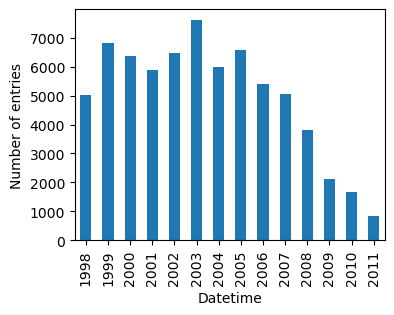
\includegraphics[width=10cm]{Amaya/datacoverage}% This is a *.eps file
	\end{center}
	\caption{ Data coverage.}\label{fig:datacoverage}
\end{figure}

\begin{figure}[h!]
	\begin{center}
		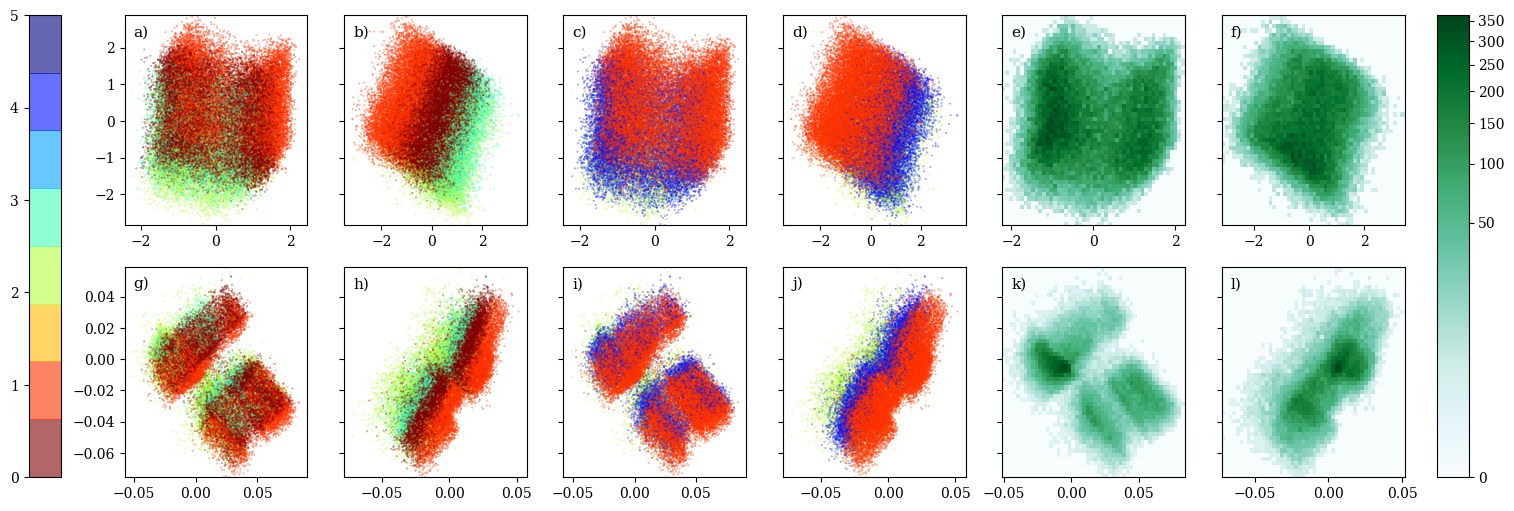
\includegraphics[width=16cm]{Amaya/dimreduc}% This is a *.eps file
	\end{center}
	\caption{ Dimension reduction. Zhao vs Xu, PCA vs AE}\label{fig:dimreduc}
\end{figure}

\begin{figure}[h!]
	\begin{center}
		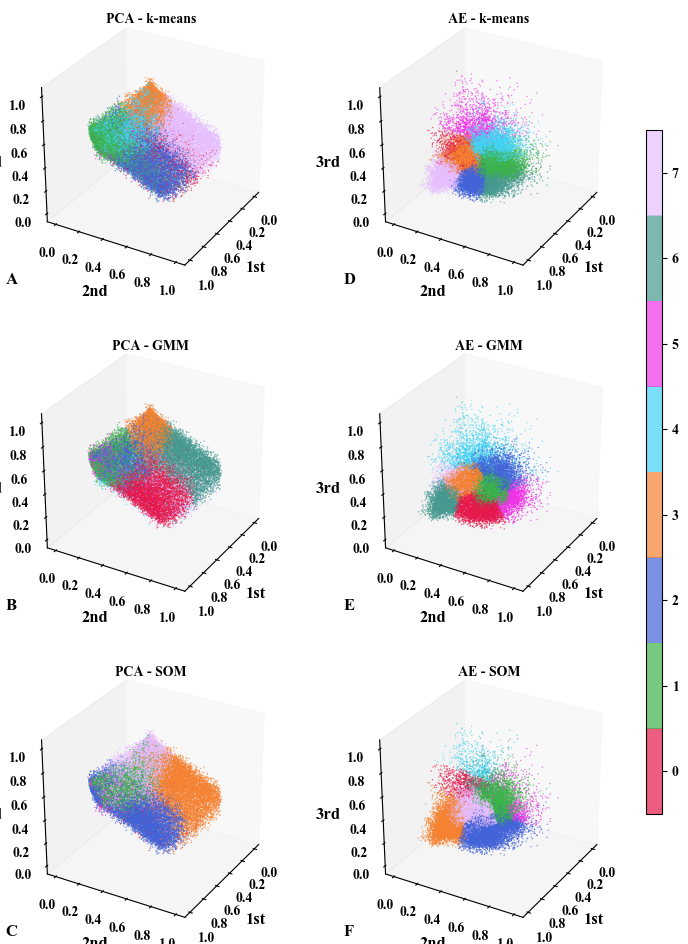
\includegraphics[width=16cm]{Amaya/clustering}% This is a *.eps file
	\end{center}
	\caption{ Clustering k-means, GMM, spectral}\label{fig:clustering}
\end{figure}

\begin{figure}[h!]
	\begin{center}
		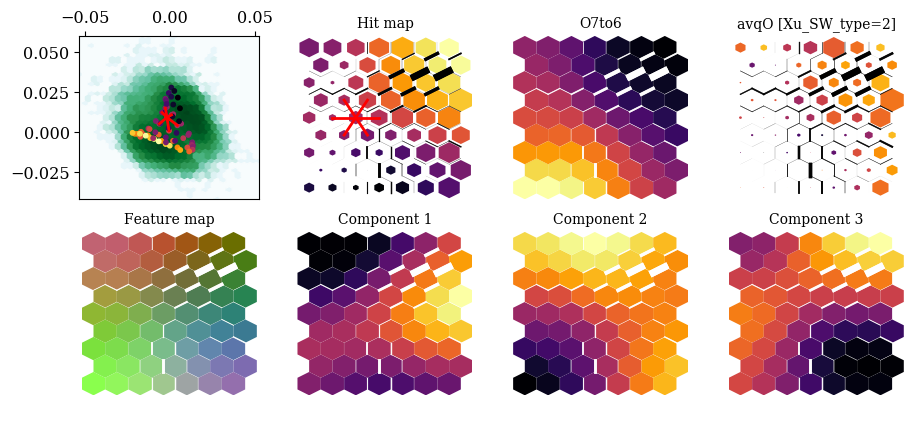
\includegraphics[width=16cm]{maps}% This is a *.eps file
	\end{center}
	\caption{ SOM Maps}\label{fig:maps}
\end{figure}

\begin{figure}[h!]
	\begin{center}
		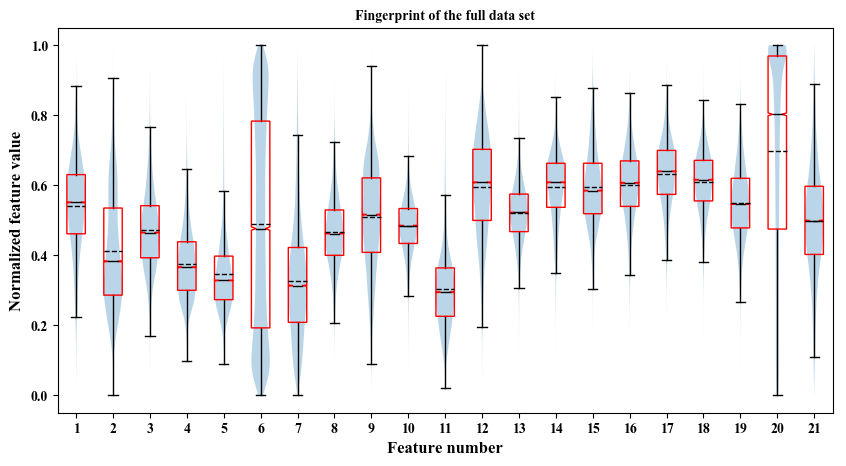
\includegraphics[width=16cm]{Amaya/datarange}% This is a *.eps file
	\end{center}
	\caption{ Data range for the Amaya et al case.}\label{fig:datarange}
\end{figure}

\end{document}
